\documentclass[11pt,a4paper]{article}

% ── Packages ──────────────────────────────────────────────────────────────────
\usepackage[utf8]{inputenc}
\usepackage[T1]{fontenc}
\usepackage{amsmath,amssymb}
\usepackage{graphicx}
\usepackage{booktabs}
\usepackage{multirow}
\usepackage{hyperref}
\usepackage[margin=1in]{geometry}
\usepackage{natbib}
\usepackage{caption}
\usepackage{subcaption}
\usepackage{float}
\usepackage{xcolor}
\usepackage{enumitem}
\usepackage{array}
\usepackage{tabularx}

\hypersetup{
  colorlinks=true,
  linkcolor=blue!60!black,
  citecolor=blue!60!black,
  urlcolor=blue!60!black
}

\graphicspath{{figures/}}

\title{
  \textbf{Can Transformers Hear Genre Through Lyrics Alone?}\\[6pt]
  \large A Comparative Study of Encoder-Only, Decoder-Only, and\\
  Encoder-Decoder Architectures with Interpretability Analysis
}
\author{
  Junho Hong\\
  \textit{STAT 359 --- Final Project}\\
  \texttt{hjunho@u.northwestern.edu}
}
\date{March 2026}

\begin{document}

\maketitle

% ══════════════════════════════════════════════════════════════════════════════
\begin{abstract}
We investigate how well transformer models can classify music genre from
song lyrics alone, comparing three architectural paradigms---encoder-only
(RoBERTa-base), decoder-only (GPT-2), and encoder-decoder
(T5-small)---all fine-tuned with Low-Rank Adaptation (LoRA).
On a balanced five-genre dataset (Rap, Pop, Rock, Country, R\&B;
$n \approx 10{,}000$), RoBERTa achieves the highest macro~F1 of 0.611,
followed by GPT-2 (0.591) and T5 (0.463), though these rankings are
confounded by differences in base model size and classification head
capacity that we analyze in detail.
All approaches plateau well below perfect accuracy, prompting the central
question of this work: \emph{why?}
We answer with four converging interpretability analyses on RoBERTa:
(1)~layer probing shows genre information saturates by layer~7 of~12,
indicating a representational ceiling;
(2)~contrastive Integrated Gradients reveal that model confusion tracks
genuine lexical ambiguity between similar genres;
(3)~embedding visualizations show Pop, Rock, and R\&B representations
are heavily interleaved;
and (4)~an independent genre similarity analysis using Sentence-BERT
finds that Pop--Rock centroid cosine similarity reaches 0.979.
External validation from zero-shot Claude~Opus (F1\,=\,0.636)
corroborates the ceiling.
These findings establish that lyrics-only genre classification is
inherently bounded at approximately F1\,$\approx$\,0.65---a data-driven
ceiling requiring multimodal features to overcome.
\end{abstract}

% ══════════════════════════════════════════════════════════════════════════════
\section{Introduction}
\label{sec:intro}

Music genre classification is a foundational task in music information
retrieval (MIR) with direct applications in streaming recommendation,
content moderation, and musicological research.
While genre has traditionally been defined by auditory
characteristics---tempo, instrumentation, harmonic structure---song
lyrics provide a complementary textual signal that captures thematic and
linguistic patterns unique to each genre.

The emergence of large pretrained language models has opened new avenues
for text classification.
However, genre classification from lyrics presents a distinctive
challenge: genres are socially constructed categories with fuzzy
boundaries, and many songs intentionally blend genres.
A Pop ballad may share the lyrical themes of a Country song, while an
R\&B track may employ vocabulary similar to Rap.
This raises two questions: \emph{how well can transformers classify genre
from lyrics alone?} And when performance plateaus, is the bottleneck
the model or the data?

We address these questions in two stages.
First, we conduct a controlled comparison of three transformer
paradigms---RoBERTa (encoder-only), GPT-2 (decoder-only), and T5
(encoder-decoder)---using LoRA adapters \citep{hu2022lora} with matched
adapter budgets but architecture-specific total trainable counts
(0.59--1.18M).
All three models plateau at similar F1 levels (0.46--0.61), well below
perfect accuracy.
Second, rather than chasing incremental improvements, we investigate
\emph{why} the plateau exists.
Through interpretability analyses on RoBERTa---layer probing,
contrastive Integrated Gradients, embedding visualization---combined
with an external genre similarity analysis and zero-shot LLM baselines,
we show that the ceiling is \emph{data-driven} (genres genuinely
overlap in lyric content) rather than model-driven.

Our contributions are:
\begin{itemize}[leftmargin=*,itemsep=2pt]
\item A controlled comparison of three transformer paradigms for
  lyrics-based genre classification under LoRA fine-tuning, with
  transparent reporting of confounds (head size, base model size) that
  complicate direct architectural comparison.
\item Interpretability evidence explaining \emph{why} performance
  plateaus: layer probing reveals representational saturation at
  mid-depth; contrastive attribution shows errors arise from genuine
  lyrical ambiguity; and embedding visualizations confirm confused
  genres are interleaved in representation space.
\item Converging external evidence that the text-only ceiling is
  approximately F1\,$\approx$\,0.65: genre centroid similarity of
  0.979 (Pop--Rock), heavily overlapping within/between-genre
  similarity distributions, and a Claude~Opus zero-shot baseline of
  only 0.636.
\end{itemize}


% ══════════════════════════════════════════════════════════════════════════════
\section{Related Work}
\label{sec:related}

\paragraph{Music Genre Classification.}
Early approaches to genre classification relied on handcrafted audio
features such as Mel-frequency cepstral coefficients (MFCCs), spectral
centroid, and tempo \citep{tzanetakis2002musical}.
Lyrics-based methods initially used bag-of-words and TF-IDF
representations with traditional classifiers
\citep{fell2014lyrics}.
\citet{tsaptsinos2017lyrics} applied hierarchical attention networks
to lyrics, demonstrating that deep learning could surpass hand-engineered
features for this task.
More recent work has combined audio and text modalities
\citep{oramas2018multimodal}, though lyrics-only classification remains
an active area due to its accessibility and interpretability.

\paragraph{Transformers for Text Classification.}
BERT \citep{devlin2019bert} and its variants have become the dominant
paradigm for text classification.
RoBERTa \citep{liu2019roberta} improved upon BERT through extended
pretraining and dynamic masking.
Decoder-only models like GPT-2 \citep{radford2019language} have been
adapted for classification via sequence-level pooling, while
encoder-decoder models like T5 \citep{raffel2020exploring} reframe
classification as text-to-text generation.
Direct comparisons across all three paradigms for the same
classification task remain relatively scarce.

\paragraph{Parameter-Efficient Fine-Tuning.}
Full fine-tuning of large language models is computationally expensive
and prone to overfitting on small datasets.
Low-Rank Adaptation (LoRA) \citep{hu2022lora} addresses this by
injecting trainable low-rank matrices into attention layers while
freezing pretrained weights, enabling roughly matched trainable
parameter budgets across models of different sizes.

\paragraph{Probing and Interpretability.}
Probing classifiers \citep{conneau2018probing} have become the standard
tool for analyzing what information is encoded at each layer of a
pretrained model.
\citet{tenney2019bert} showed that BERT's layers recapitulate the
classical NLP pipeline, with syntactic information peaking in middle
layers and semantic information in later layers.
For token-level attribution, Integrated Gradients
\citep{sundararajan2017axiomatic} provides axiomatic guarantees of
completeness and sensitivity.

\paragraph{Zero-Shot LLM Classification.}
The in-context learning paradigm introduced by GPT-3
\citep{brown2020language} enables large language models to perform
classification without task-specific training.
We use zero-shot LLM evaluation as a reference point that provides an
upper bound on the information accessible from lyrics plus world
knowledge.


% ══════════════════════════════════════════════════════════════════════════════
\section{Dataset}
\label{sec:data}

\subsection{Data Collection and Preprocessing}

We source song lyrics from the \texttt{genius-song-lyrics} dataset on
Hugging Face \citep{genius_dataset}, which contains 2.76 million songs
with lyrics and genre metadata scraped from Genius.com.
We retain five genres: \textbf{Rap/Hip-Hop}, \textbf{Pop},
\textbf{Rock}, \textbf{Country}, and \textbf{R\&B}.
The preprocessing pipeline:

\begin{enumerate}[leftmargin=*,itemsep=2pt]
\item \textbf{Language filtering:} Retain only English-language songs,
  requiring agreement between CLD3 and fastText detectors.
\item \textbf{Stratified sampling:} Sample 2{,}000 songs per genre
  (2{,}500 for Pop to offset higher noise) for the comparison
  experiment.
  A larger set of 5{,}000 per genre (6{,}000 for Pop) is used for
  interpretability analyses.
  All sampling uses seed~42.
\item \textbf{Lyric cleaning:} Remove structural annotations
  (e.g., \texttt{[Verse]}, \texttt{[Chorus]}) via regex, collapse
  excessive whitespace, and truncate to 2{,}000 characters.
\item \textbf{Minimum length filter:} Discard songs with fewer than
  20 words after cleaning.
\item \textbf{Stratified splitting:} 80/10/10
  train/validation/test split with stratification by label.
  Validation and test sets are further balanced to equal counts per
  class.
\end{enumerate}

\noindent
The resulting comparison dataset contains approximately 8{,}000
training, 1{,}000 validation, and 1{,}000 test samples.

\subsection{Exploratory Data Analysis}
\label{sec:eda}

\begin{figure}[t]
  \centering
  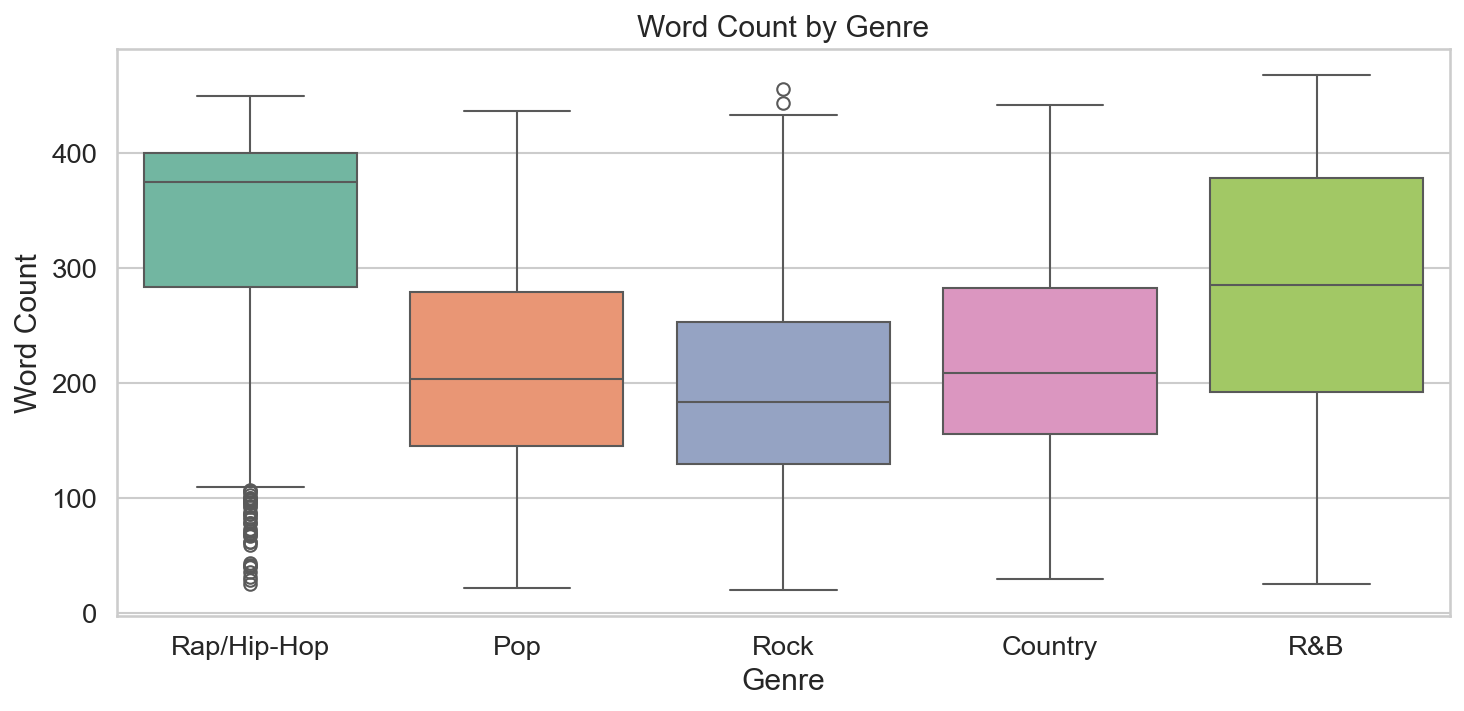
\includegraphics[width=\textwidth]{word_count_boxplot.png}
  \caption{Word count distributions by genre. Rap lyrics are
  substantially longer (median 375 words) than Rock (184) or Pop (204),
  reflecting the density of rap verses. All models receive the same
  512-token truncated inputs.}
  \label{fig:wordcount}
\end{figure}

Figure~\ref{fig:wordcount} shows substantial variation in lyric length
across genres.
Rap lyrics are the longest (mean 333 words), while Rock are the shortest
(mean 196 words).
This length disparity could serve as a confounding feature; however,
tokenizer truncation at 512 tokens bounds the effective input length.

\begin{figure}[t]
  \centering
  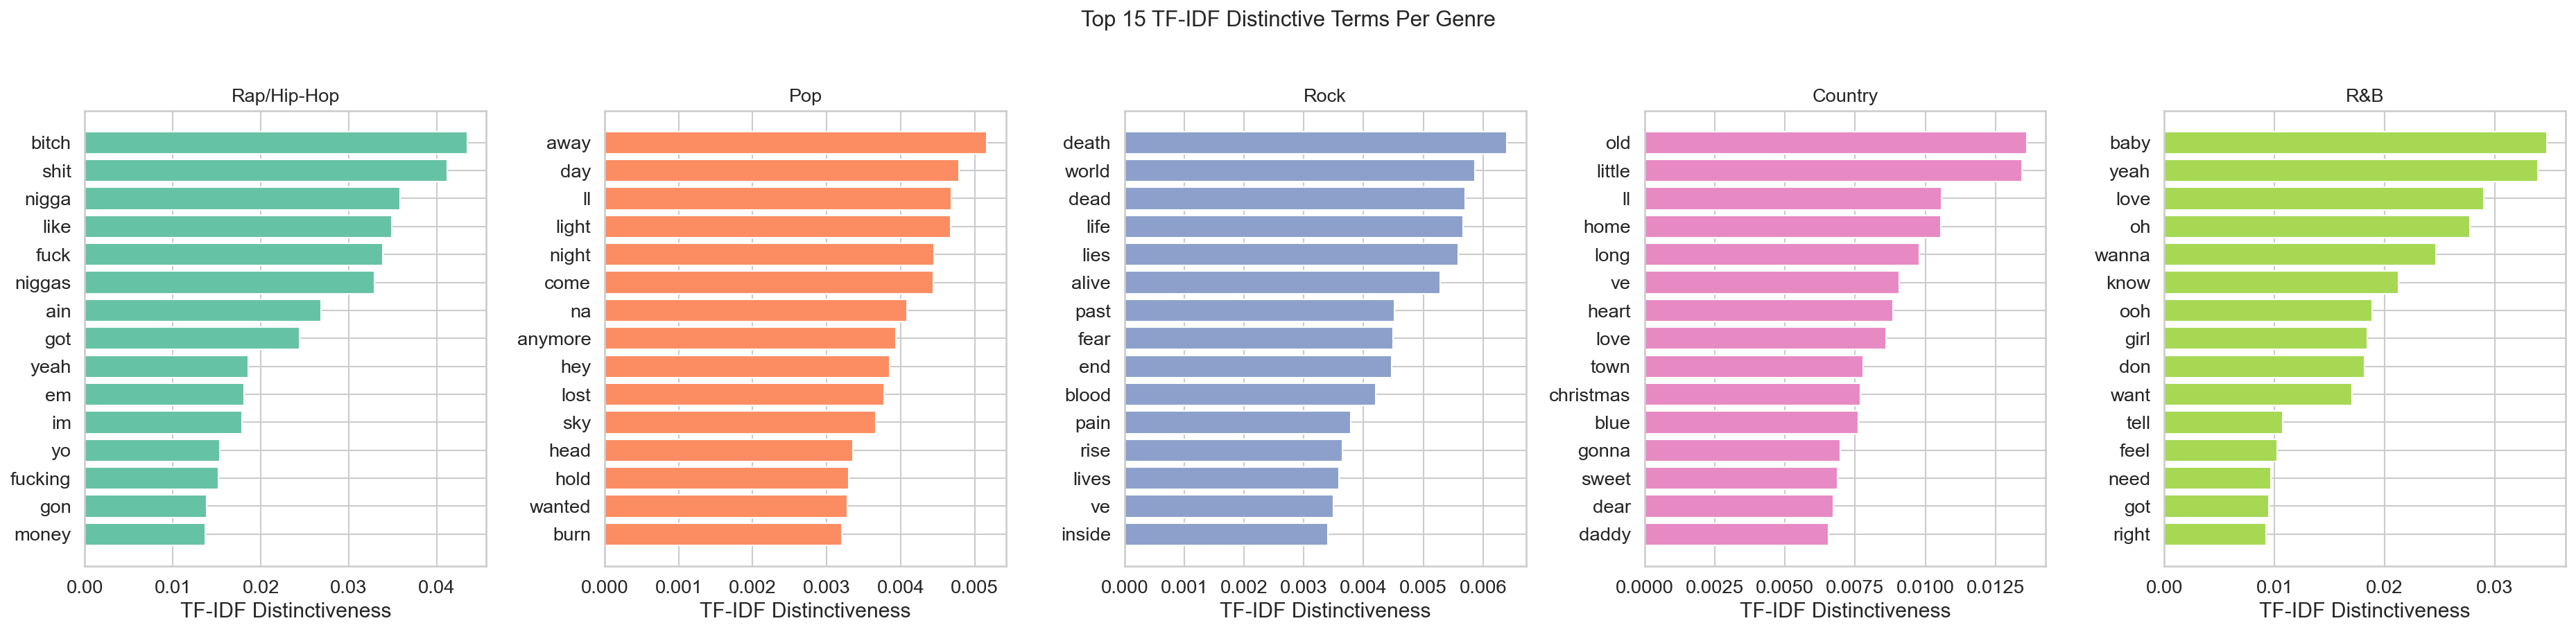
\includegraphics[width=\textwidth]{tfidf_distinctive_terms.png}
  \caption{Top 15 TF-IDF distinctive terms per genre, computed as the
  difference between a genre's mean TF-IDF vector and the complement's
  mean. Pop has the weakest distinctive terms, foreshadowing its role
  as the most-confused class.}
  \label{fig:tfidf}
\end{figure}

TF-IDF analysis (Figure~\ref{fig:tfidf}) reveals that each genre
possesses a distinctive vocabulary:
Rap is characterized by explicit language and slang; Rock by themes of
darkness and pain; Country by domestic and rural imagery (\emph{old},
\emph{home}, \emph{town}); R\&B by terms of endearment.
Notably, Pop has the weakest distinctive terms---its most characteristic
words (\emph{away}, \emph{day}, \emph{night}) are generic and shared
with other genres.

\begin{figure}[t]
  \centering
  \begin{subfigure}[b]{0.48\textwidth}
    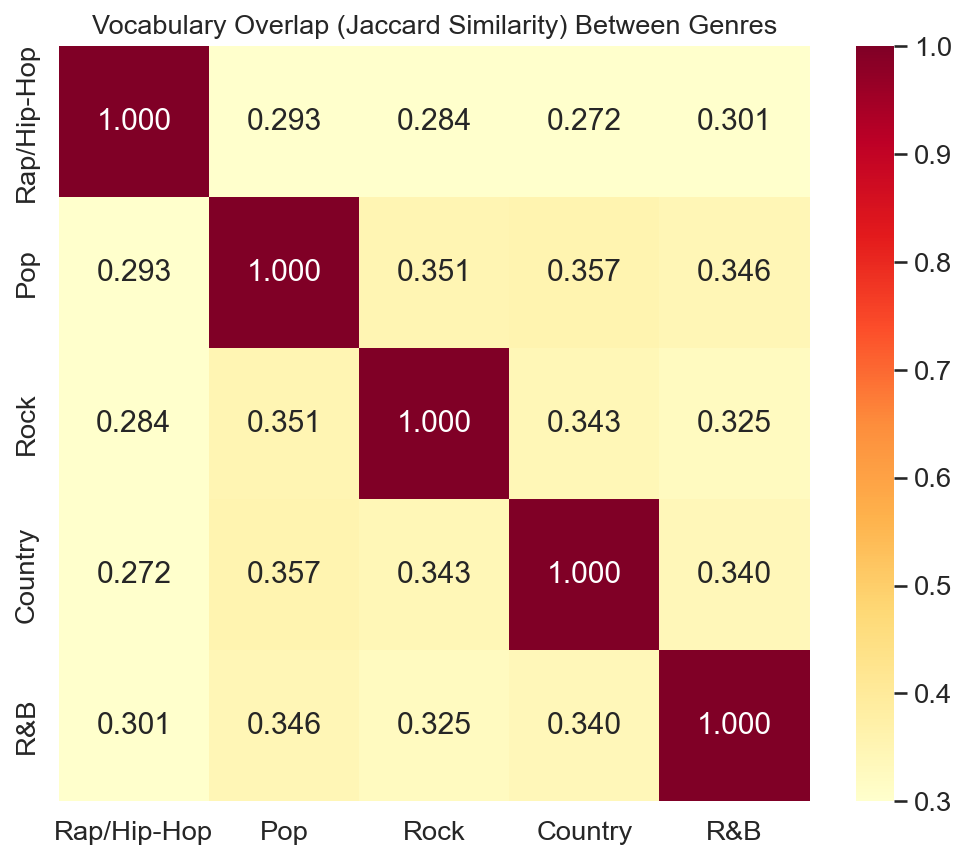
\includegraphics[width=\textwidth]{vocab_overlap_heatmap.png}
    \caption{Jaccard vocabulary overlap.}
    \label{fig:jaccard}
  \end{subfigure}
  \hfill
  \begin{subfigure}[b]{0.48\textwidth}
    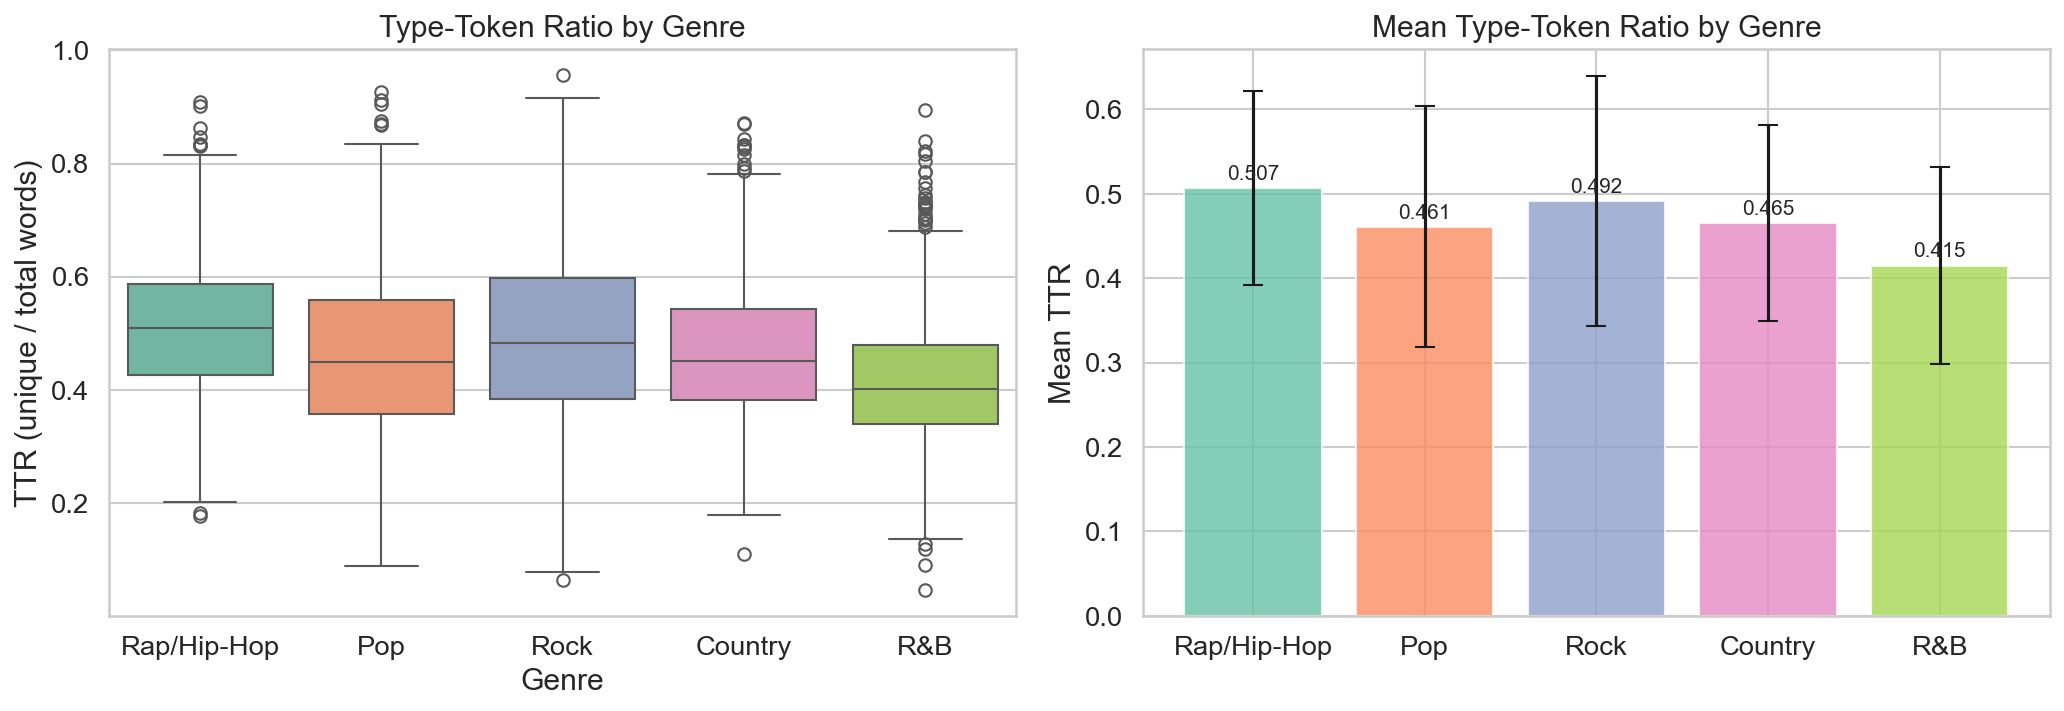
\includegraphics[width=\textwidth]{type_token_ratio.png}
    \caption{Type-token ratio by genre.}
    \label{fig:ttr}
  \end{subfigure}
  \caption{(a)~Pairwise Jaccard similarity of unique word sets per
  genre (stopwords removed). Rap shares the least vocabulary with other
  genres. (b)~Vocabulary richness: Rock and Country exhibit higher
  TTR (more diverse word choices per song).}
  \label{fig:vocab_analysis}
\end{figure}

Vocabulary overlap analysis (Figure~\ref{fig:jaccard}) confirms that
Rap has the most distinctive lexicon, while Pop, Rock, and Country
share substantial vocabulary.
These EDA findings foreshadow the classification results: genres with
more distinctive linguistic signatures are easier to classify.


% ══════════════════════════════════════════════════════════════════════════════
\section{Methods}
\label{sec:methods}

\subsection{Model Architectures}

We compare three pretrained transformer architectures:

\paragraph{RoBERTa (Encoder-Only).}
\texttt{roberta-base} (125M parameters) with a two-layer classification
head on the \texttt{[CLS]} token \citep{liu2019roberta}.
Bidirectional self-attention allows each token to attend to the full
context.

\paragraph{GPT-2 (Decoder-Only).}
\texttt{gpt2} (124M parameters) with a classification head on the
last non-padding token \citep{radford2019language}.
Causal (left-to-right) attention forces sequential representation
building; padding token is set to \texttt{eos\_token}.

\paragraph{T5 (Encoder-Decoder).}
\texttt{t5-small} (60M parameters) in text-to-text mode
\citep{raffel2020exploring}: input is
\texttt{"classify genre: <lyrics>"}, target is the genre string.
Predictions are decoded via greedy generation
(\texttt{max\_new\_tokens=8}) and mapped back to integer labels.

\subsection{Parameter-Efficient Fine-Tuning with LoRA}

All models are fine-tuned using LoRA \citep{hu2022lora}, which injects
trainable rank-$r$ decomposition matrices $\Delta W = BA$ into
selected attention projections while freezing all pretrained parameters.
Table~\ref{tab:lora} summarizes the configuration.

\begin{table}[ht]
\centering
\caption{LoRA configuration ($\alpha=32$, dropout$\,=0.1$).
Adapter parameters are matched (590K); total trainable counts differ
due to classification heads.}
\label{tab:lora}
\begin{tabular}{lccccc}
\toprule
\textbf{Model} & \textbf{Base Size} & \textbf{Targets} & \textbf{Rank}
& \textbf{Head} & \textbf{Total Trainable} \\
\midrule
RoBERTa & 125M & query, value & 16 & 594K & 1.18M \\
GPT-2 & 124M & c\_attn & 16 & 3.8K & 0.59M \\
T5 & 60M & q, v (enc.+dec.) & 16 & 0 & 0.59M \\
\midrule
RoBERTa (interp.) & 125M & query, key, value & 16 & 594K & 1.48M \\
\bottomrule
\end{tabular}
\end{table}

While the LoRA adapter parameters are identical across the comparison
models (590K), total trainable counts differ:
RoBERTa's two-layer classification head (768$\to$768$\to$5) adds 594K
parameters, GPT-2's single linear head adds only 3.8K, and T5 has no
separate head (text-to-text reuses the frozen LM head).
This asymmetry complicates direct comparison and is discussed in
Section~\ref{sec:limitations}.

\subsection{Training Procedure}

\paragraph{Optimization.}
All models are trained with AdamW \citep{loshchilov2019decoupled}
and a cosine learning rate schedule with linear warmup.
Gradient norms are clipped at 1.0.

\paragraph{Early Stopping.}
We monitor validation macro~F1 and halt if no improvement is observed
for 3 consecutive epochs (comparison) or 4 epochs (interpretability
model).
The checkpoint with the highest validation F1 is retained.

\paragraph{Interpretability Model.}
For interpretability analyses (Section~\ref{sec:interp}), we train a
separate RoBERTa on the larger dataset (5{,}000 samples/genre) with
expanded LoRA targets (query/key/value), a lower learning rate
($10^{-4}$), gradient accumulation (effective batch size~64), FP16
mixed precision, and random contiguous word cropping as data
augmentation (50--100\% of words for songs $>$100 words).
This model achieves F1\,=\,0.608 on the Phase~2 test set and
0.605 on the original test set---comparable to the comparison
RoBERTa (0.611)---confirming it is a representative subject for
interpretability.

\begin{table}[ht]
\centering
\caption{Hyperparameter settings.}
\label{tab:hyperparams}
\begin{tabular}{lcc}
\toprule
\textbf{Hyperparameter} & \textbf{Comparison} &
\textbf{Interpretability} \\
\midrule
Max sequence length & 512 & 512 \\
Batch size & 64 & 32 \\
Learning rate & $2 \times 10^{-4}$ & $1 \times 10^{-4}$ \\
Weight decay & 0.01 & 0.01 \\
Max epochs & 10 & 15 \\
Warmup ratio & 0.10 & 0.06 \\
Gradient accumulation & 1 & 2 \\
Mixed precision (FP16) & No & Yes \\
Augmentation & No & Yes \\
Samples per genre & 2{,}000 & 5{,}000 \\
\bottomrule
\end{tabular}
\end{table}

\subsection{Zero-Shot LLM Baselines}

To contextualize fine-tuned model performance, we evaluate two Claude
models \citep{anthropic2025claude_opus4, anthropic2025claude_haiku45} in a zero-shot setting following the
in-context learning paradigm of \citet{brown2020language}:
\textbf{Claude~Haiku} (smaller, faster) and \textbf{Claude~Opus}
(larger, more capable).
Each model receives a system prompt constraining output to a single
genre label, and the input is the raw lyric text (truncated to 3{,}000
characters).
We evaluate on 50 randomly sampled test songs per genre (250 total).
Unlike our fine-tuned models, these LLMs have access to world
knowledge about artists, musical styles, and cultural context, providing
a reference point for the information available beyond lyrics alone.
We note that the 250-sample evaluation introduces higher variance than
the full 1{,}000-sample test set, and treat LLM results as illustrative
rather than definitive.

\subsection{Interpretability Methods}

All interpretability analyses are conducted on the RoBERTa model
trained on the larger dataset.

\paragraph{Genre Similarity Analysis.}
To quantify task difficulty independently of our trained models, we
encode all lyrics using a sentence-transformer
(\texttt{all-MiniLM-L6-v2}; \citealp{reimers2019sentence}) and compute
pairwise centroid cosine similarities between genres.
Higher inter-genre similarity implies harder classification.
We also compare within-genre and between-genre pairwise similarity
distributions to assess the degree of class overlap.

\paragraph{Layer Probing.}
Following \citet{conneau2018probing} and \citet{tenney2019bert}, we
extract the \texttt{[CLS]} embedding from each of the 13 layers
(layer~0 = static embeddings; layers~1--12 = transformer outputs) and
train a multinomial logistic regression classifier
(L-BFGS solver, $C=1.0$, max 1{,}000 iterations) on the training set.
Test-set macro~F1 at each layer quantifies linearly accessible genre
information at that depth.
We note that probing accuracy is a lower bound on the information
present, since it reflects only what a linear classifier can extract.

\paragraph{Embedding Visualization.}
We extract \texttt{[CLS]} embeddings from the final transformer layer
and project them to 2D using t-SNE
\citep{vandermaaten2008visualizing} (perplexity~30, 1{,}000 iterations)
and UMAP \citep{mcinnes2018umap} ($k=15$, min\_dist$\,=0.1$).
These projections are qualitative; we avoid over-interpreting cluster
boundaries given the stochastic nature of both methods.

\paragraph{Contrastive Integrated Gradients.}
For the top confused genre pairs (identified from the confusion matrix),
we apply Integrated Gradients \citep{sundararajan2017axiomatic}
(implemented via Captum) with a
\emph{contrastive} objective: attributions are computed with respect to
the logit difference $f_A(\mathbf{x}) - f_B(\mathbf{x})$ between two
confused classes $A$ and $B$.
This reveals which tokens push the model toward one genre over the
other---a more informative signal than standard single-class IG when
genres share substantial vocabulary.
We use 30 interpolation steps per sample and aggregate contrastive
vocabularies across 30 samples per pair.


% ══════════════════════════════════════════════════════════════════════════════
\section{Results}
\label{sec:results}

\subsection{Architecture Comparison}

\begin{table}[t]
\centering
\caption{Test-set performance. Fine-tuned models are evaluated on the
full 1{,}000-sample test set. LLM baselines use a 250-sample subset
(50~per genre). All scores are single-run point estimates; see
Section~\ref{sec:limitations} for discussion of variance.}
\label{tab:results}
\begin{tabular}{llccc}
\toprule
\textbf{Model} & \textbf{Type} & \textbf{Accuracy} &
\textbf{F1 Macro} & \textbf{F1 Weighted} \\
\midrule
RoBERTa & Fine-tuned & 0.613 & \textbf{0.611} & 0.611 \\
GPT-2 & Fine-tuned & 0.604 & 0.591 & 0.591 \\
T5 & Fine-tuned & 0.454 & 0.463 & 0.463 \\
\midrule
Claude Haiku & Zero-shot LLM & 0.596 & 0.584 & 0.587 \\
Claude Opus & Zero-shot LLM & \textbf{0.649} & \textbf{0.636} & 0.639 \\
\midrule
\textit{Random} & \textit{Baseline} & \textit{0.200} & \textit{0.200}
& \textit{0.200} \\
\bottomrule
\end{tabular}
\end{table}

Table~\ref{tab:results} summarizes all results.
Among the fine-tuned models, \textbf{RoBERTa achieves the highest
macro~F1 of 0.611}, followed by GPT-2 (0.591) and T5 (0.463).
However, this ranking must be interpreted with caution due to several
confounds:

\begin{itemize}[leftmargin=*,itemsep=1pt]
\item RoBERTa's advantage over GPT-2 (2~points~F1) is modest and may
  be partly attributable to its larger trainable classification head
  (594K vs.~3.8K), providing $150\times$ more task-specific capacity.
\item T5's larger gap ($-$15~points) likely reflects a combination of
  its smaller base model (\texttt{t5-small} at 60M vs.\ 125M), the
  additional difficulty of the text-to-text formulation (where decoding
  errors further degrade performance), and the absence of a trainable
  classification head.
\end{itemize}

\noindent
We emphasize that the ranking
RoBERTa~$>$~GPT-2~$\gg$~T5 reflects the \emph{full experimental
setup} (architecture + head + base model size), not purely
architectural differences.
We revisit these confounds in Section~\ref{sec:limitations}.

\begin{figure}[t]
  \centering
  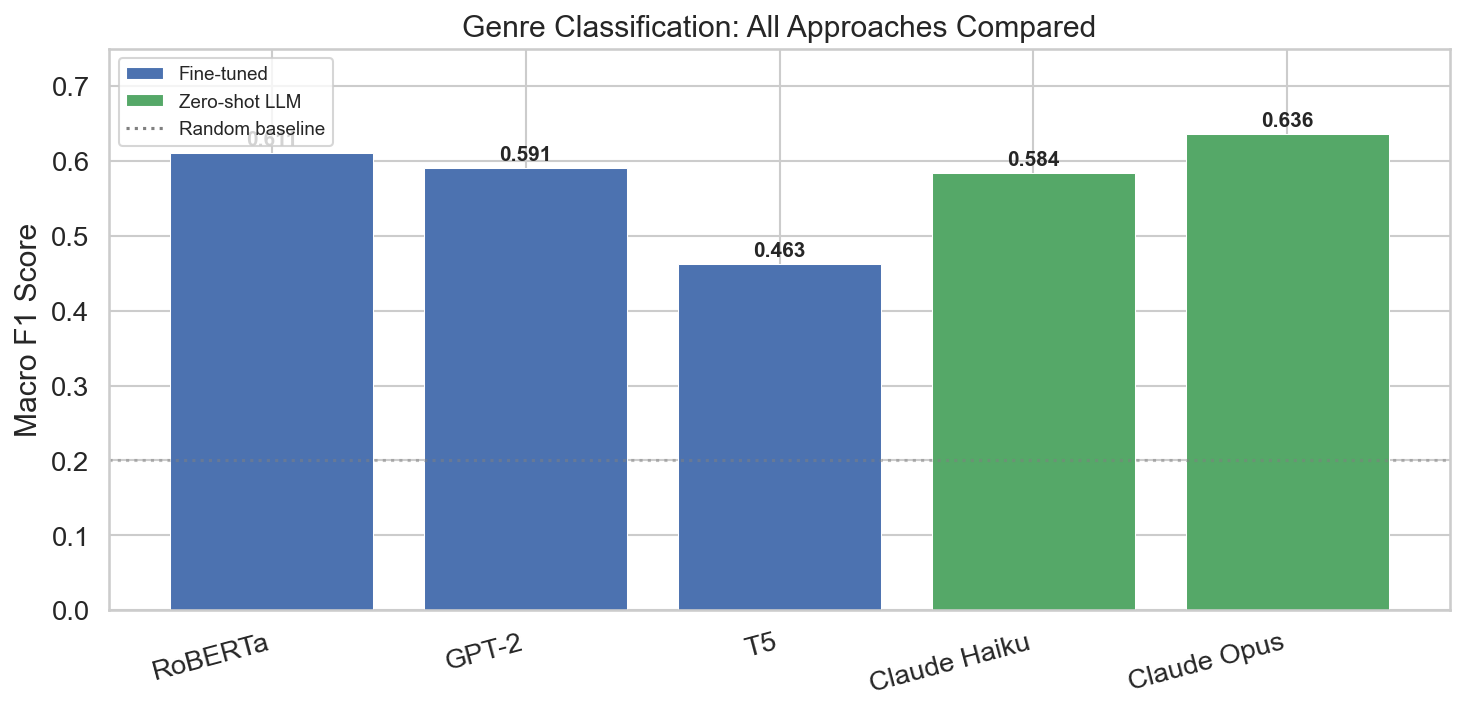
\includegraphics[width=\textwidth]{unified_comparison.png}
  \caption{Macro F1 across all approaches. The random baseline is 0.200.
  All approaches cluster between 0.46--0.64, with Claude Opus setting a
  soft upper bound at 0.636.}
  \label{fig:unified}
\end{figure}

Figure~\ref{fig:unified} visualizes the clustering of all approaches
in the 0.46--0.64 F1 range, well above the random baseline (0.200) but
well below perfect classification.

\subsection{Training Dynamics}

\begin{figure}[t]
  \centering
  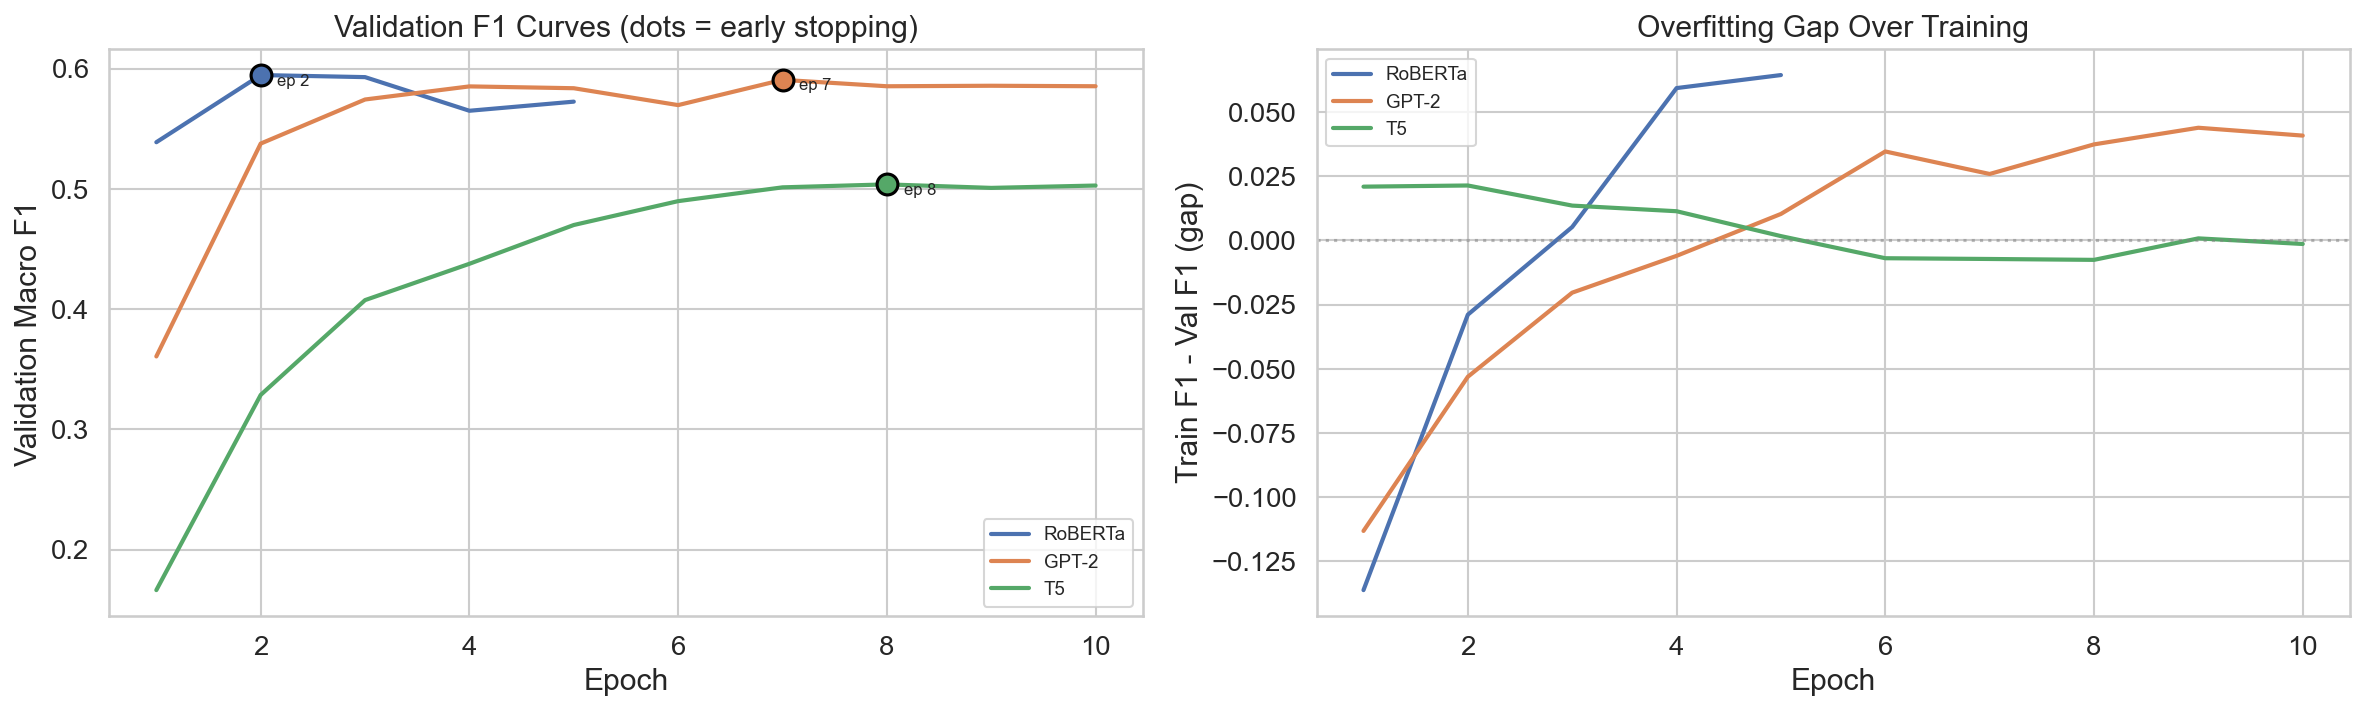
\includegraphics[width=\textwidth]{training_dynamics.png}
  \caption{Left: validation F1 curves with early stopping points (dots).
  RoBERTa peaks at epoch~2; GPT-2 at epoch~7. Right: train--val F1
  gap. RoBERTa and GPT-2 overfit progressively; T5 shows minimal
  gap, suggesting underfitting.}
  \label{fig:dynamics}
\end{figure}

Figure~\ref{fig:dynamics} reveals distinct training behaviors.
RoBERTa converges rapidly, reaching peak validation F1 by epoch~2,
consistent with bidirectional attention's efficiency at capturing
document-level features.
GPT-2 requires 7 epochs, consistent with the need for its causal
mechanism to gradually build useful representations from left to right.
T5 shows the slowest convergence and smallest train--val gap,
suggesting it \emph{underfits}---the seq2seq objective adds
optimization difficulty that 10 epochs cannot overcome.

\subsection{Confusion Analysis}

\begin{figure}[t]
  \centering
  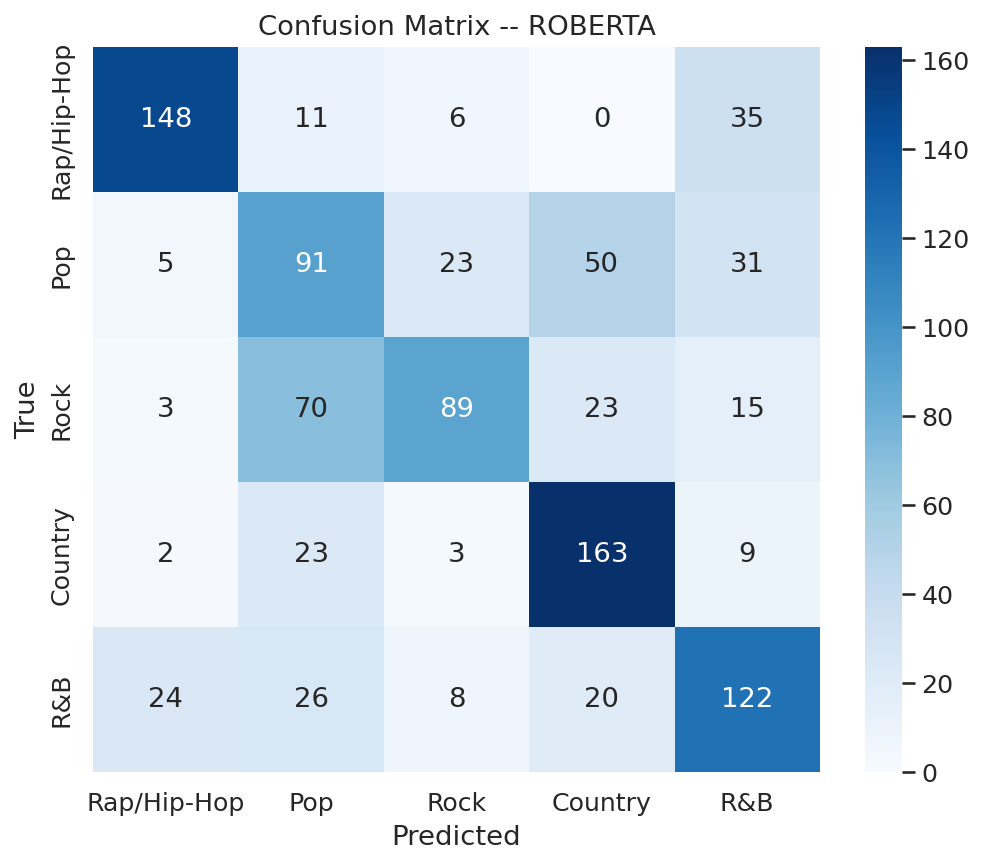
\includegraphics[width=0.55\textwidth]{cm_roberta.png}
  \caption{RoBERTa confusion matrix (1{,}000 test samples, 200 per genre).
  Country is best-classified (163/200); Pop is most confused, with
  errors spreading to Rock (23), Country (50), and R\&B (31).}
  \label{fig:cm}
\end{figure}

The confusion matrix (Figure~\ref{fig:cm}) reveals systematic patterns.
Country is the best-classified genre (82\% accuracy), benefiting from
distinctive rural themes, while Rap achieves 74\% accuracy due to its
unique vocabulary.
The largest confusion clusters are \textbf{Rock$\to$Pop} (70 errors)
and \textbf{Pop$\to$Country} (50 errors)---precisely the genre pairs
with the highest semantic similarity, as we quantify next.


% ══════════════════════════════════════════════════════════════════════════════
\section{Understanding the Performance Ceiling}
\label{sec:interp}

All three fine-tuned models plateau at F1\,$\leq$\,0.61, and even
Claude~Opus achieves only 0.636.
This section investigates \emph{why} the ceiling exists through
four complementary analyses, ordered from the data level
(genre similarity) through model behavior (error correlation,
embeddings, probing) to token-level explanations
(contrastive attribution).

\subsection{Genre Similarity: The Task Is Inherently Hard}

\begin{figure}[t]
  \centering
  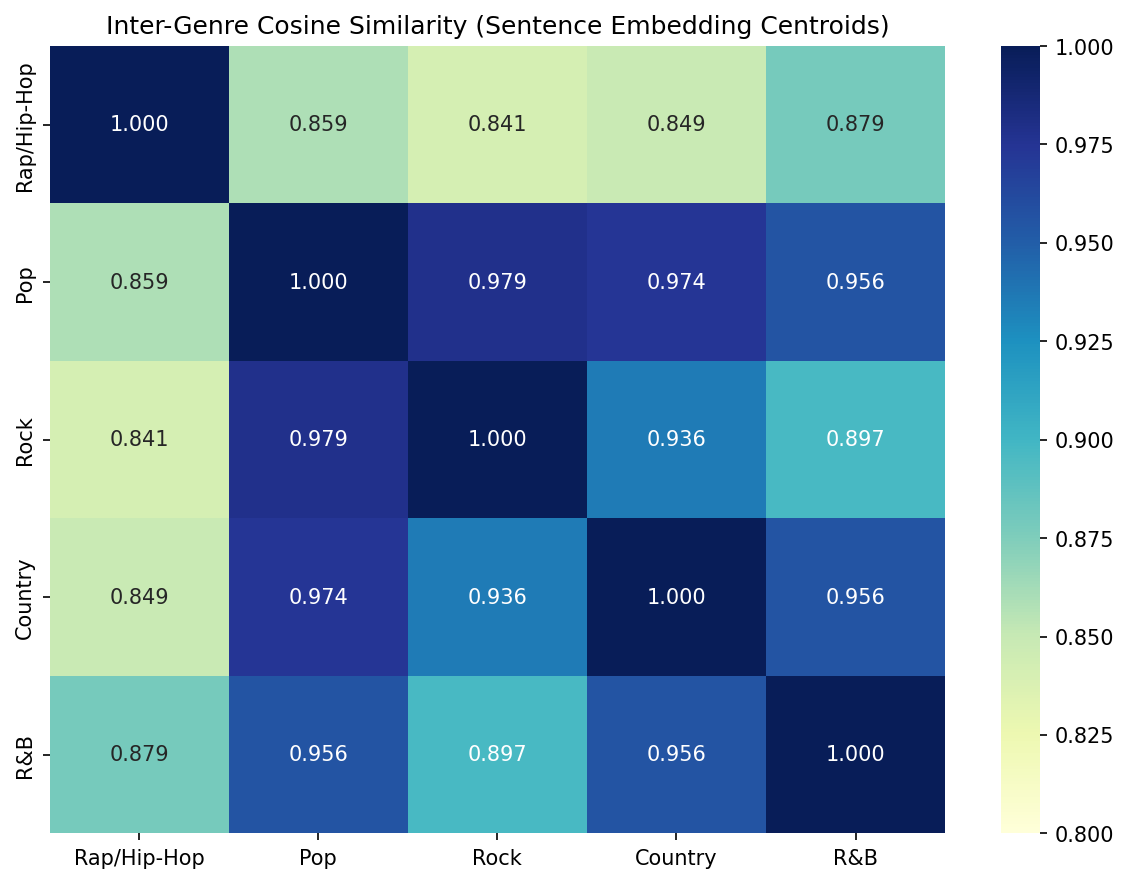
\includegraphics[width=0.6\textwidth]{genre_centroid_similarity.png}
  \caption{Inter-genre cosine similarity of Sentence-BERT embedding
  centroids. Pop--Rock (0.979) and Pop--Country (0.974) are nearly
  indistinguishable, while Rap is the most distinct genre.}
  \label{fig:centroid_sim}
\end{figure}

Using Sentence-BERT \citep{reimers2019sentence} as an independent
embedding model (not our fine-tuned RoBERTa), we find that most genre
pairs have centroid cosine similarity above 0.85
(Figure~\ref{fig:centroid_sim}).
Pop--Rock reaches 0.979 and Pop--Country 0.974---nearly identical in
semantic space.
Only Rap stands apart (0.84--0.88 with other genres).

\begin{figure}[t]
  \centering
  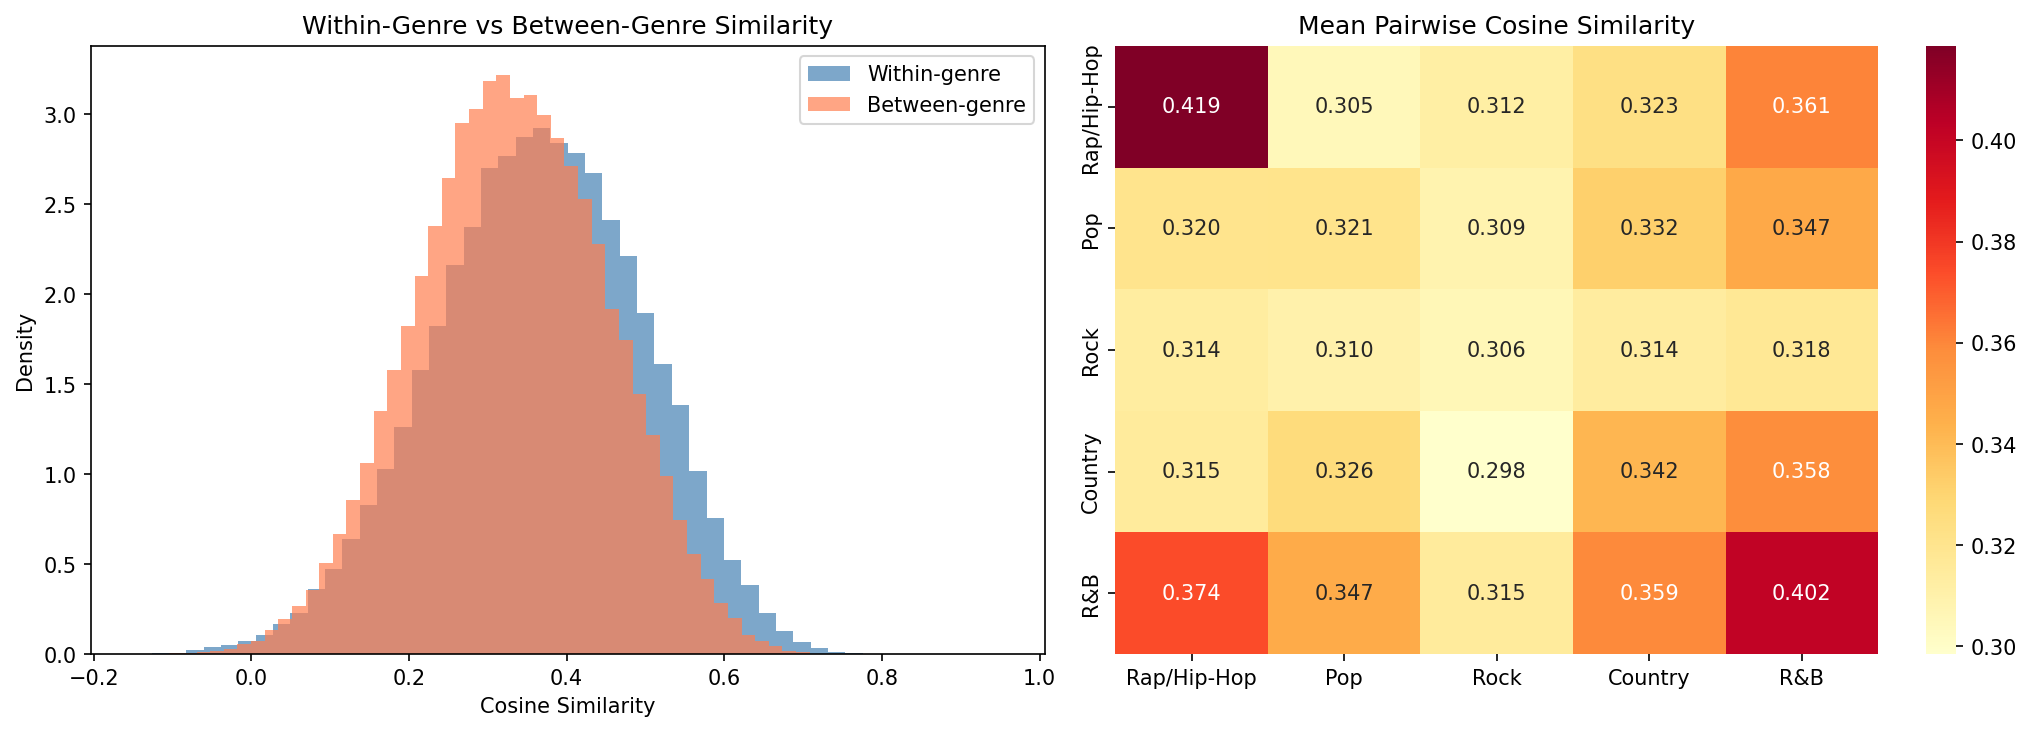
\includegraphics[width=\textwidth]{genre_similarity_analysis.png}
  \caption{Left: within-genre ($\mu = 0.363$) and between-genre
  ($\mu = 0.331$) pairwise similarity distributions overlap almost
  entirely. Right: mean pairwise cosine similarity matrix at the
  sample level.}
  \label{fig:sim_distributions}
\end{figure}

At the sample level (Figure~\ref{fig:sim_distributions}), within-genre
and between-genre similarity distributions overlap heavily
(means 0.363 vs.\ 0.331).
This means a given Pop song is often more similar to a random Rock song
than to another Pop song---a fundamental constraint on any lyrics-only
classifier.

\subsection{Error--Similarity Correlation: Confusion Mirrors Reality}

\begin{figure}[t]
  \centering
  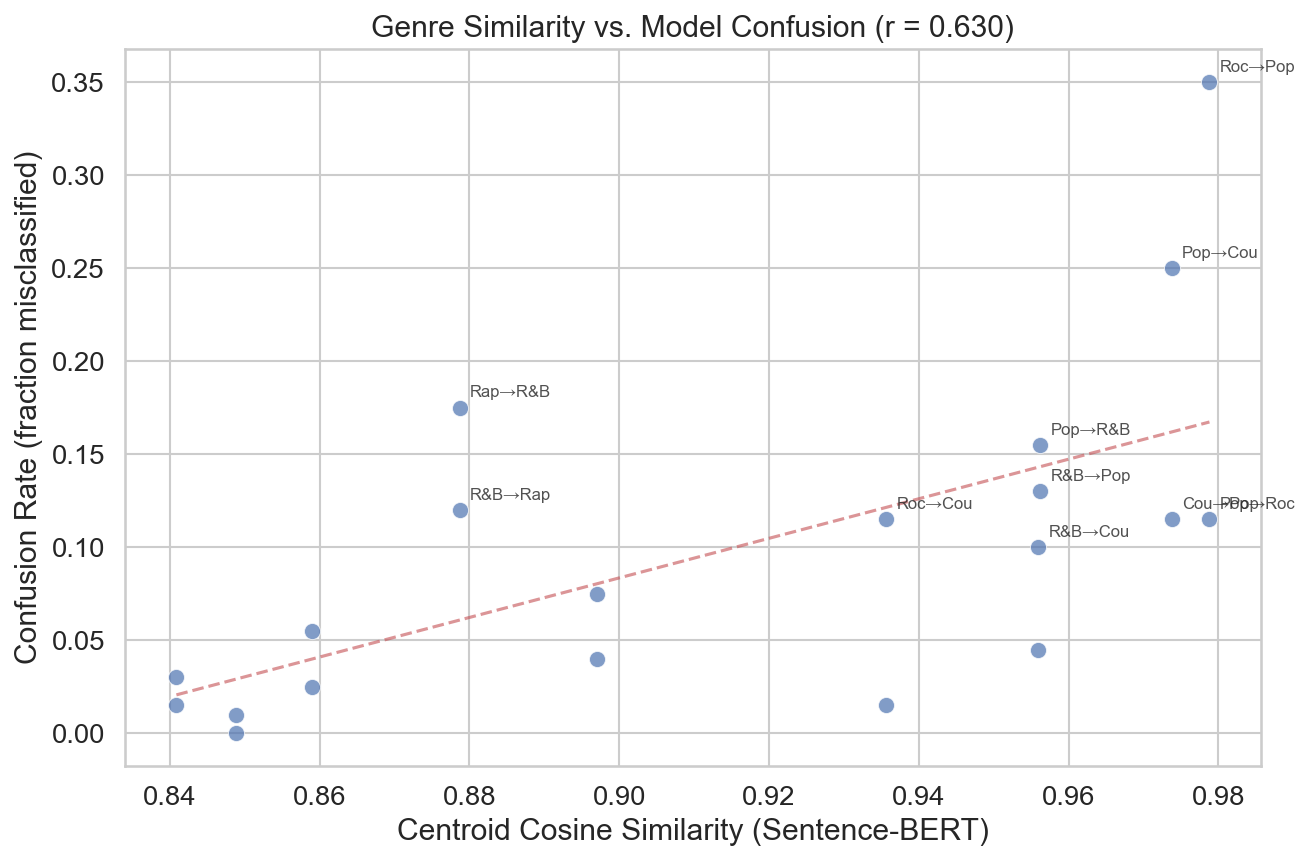
\includegraphics[width=0.7\textwidth]{error_vs_similarity.png}
  \caption{Genre centroid similarity vs.\ RoBERTa confusion rate for
  all 20 directed genre pairs (Pearson $r = 0.630$). The most-confused
  pairs are also the most semantically similar.}
  \label{fig:error_sim}
\end{figure}

We connect genre similarity to model behavior by plotting centroid
cosine similarity against RoBERTa's confusion rate for each directed
genre pair (Figure~\ref{fig:error_sim}).
The Pearson correlation is $r = 0.630$: genres that are more
semantically similar are confused more frequently.
The three highest confusion rates are:
\begin{itemize}[leftmargin=*,itemsep=1pt]
\item Rock$\to$Pop: 35\% confusion, similarity 0.979
\item Pop$\to$Country: 25\% confusion, similarity 0.974
\item Rap$\to$R\&B: 17.5\% confusion, similarity 0.879
\end{itemize}

\noindent
Conversely, Rap$\to$Country has 0\% confusion and only 0.849
similarity.
This establishes that model errors are not random but reflect genuine
semantic proximity---the model is \emph{rationally confused}.

\subsection{Embedding Visualization: Confirming the Overlap}

\begin{figure}[t]
  \centering
  \begin{subfigure}[b]{0.48\textwidth}
    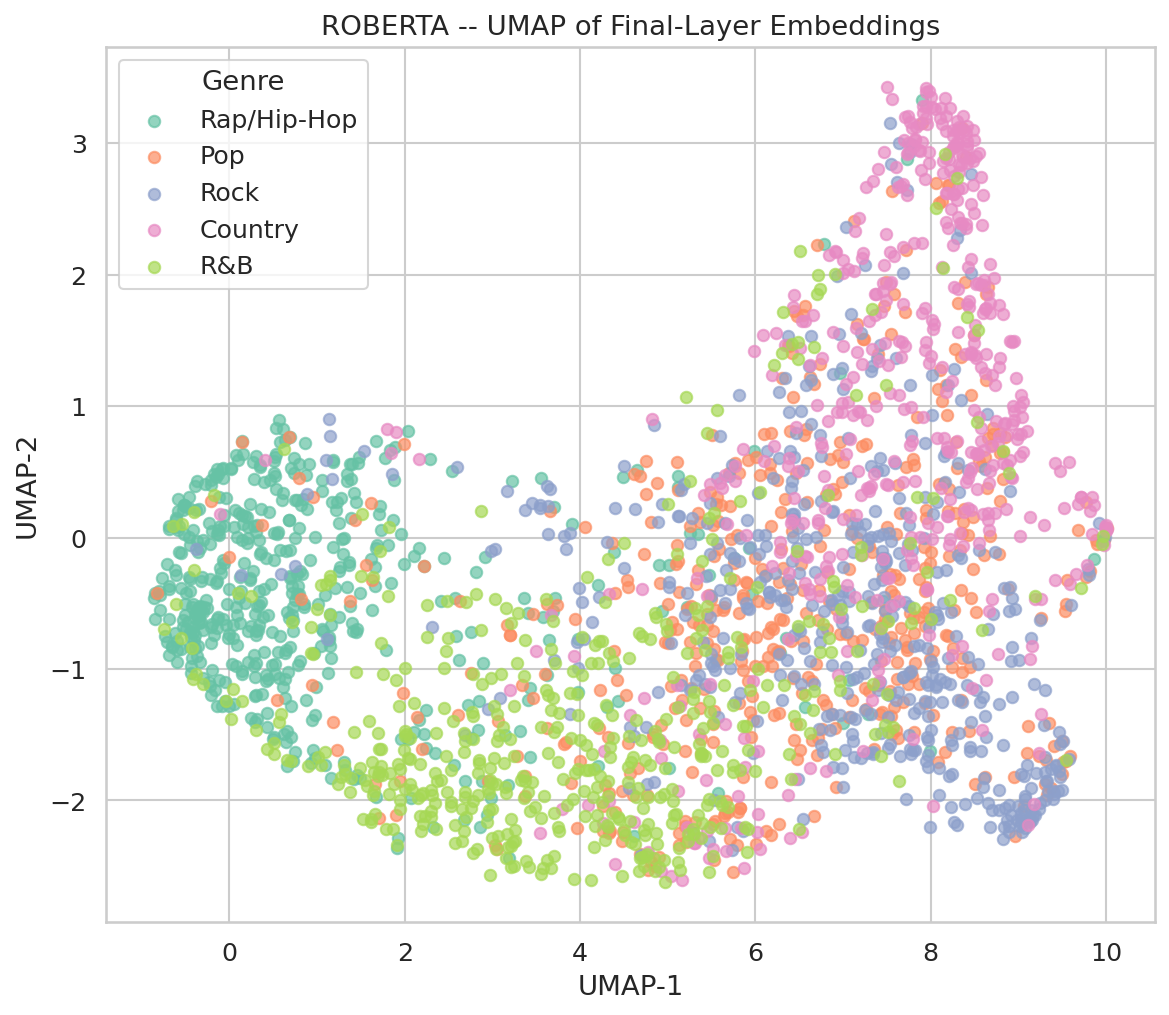
\includegraphics[width=\textwidth]{umap_roberta.png}
    \caption{UMAP projection.}
  \end{subfigure}
  \hfill
  \begin{subfigure}[b]{0.48\textwidth}
    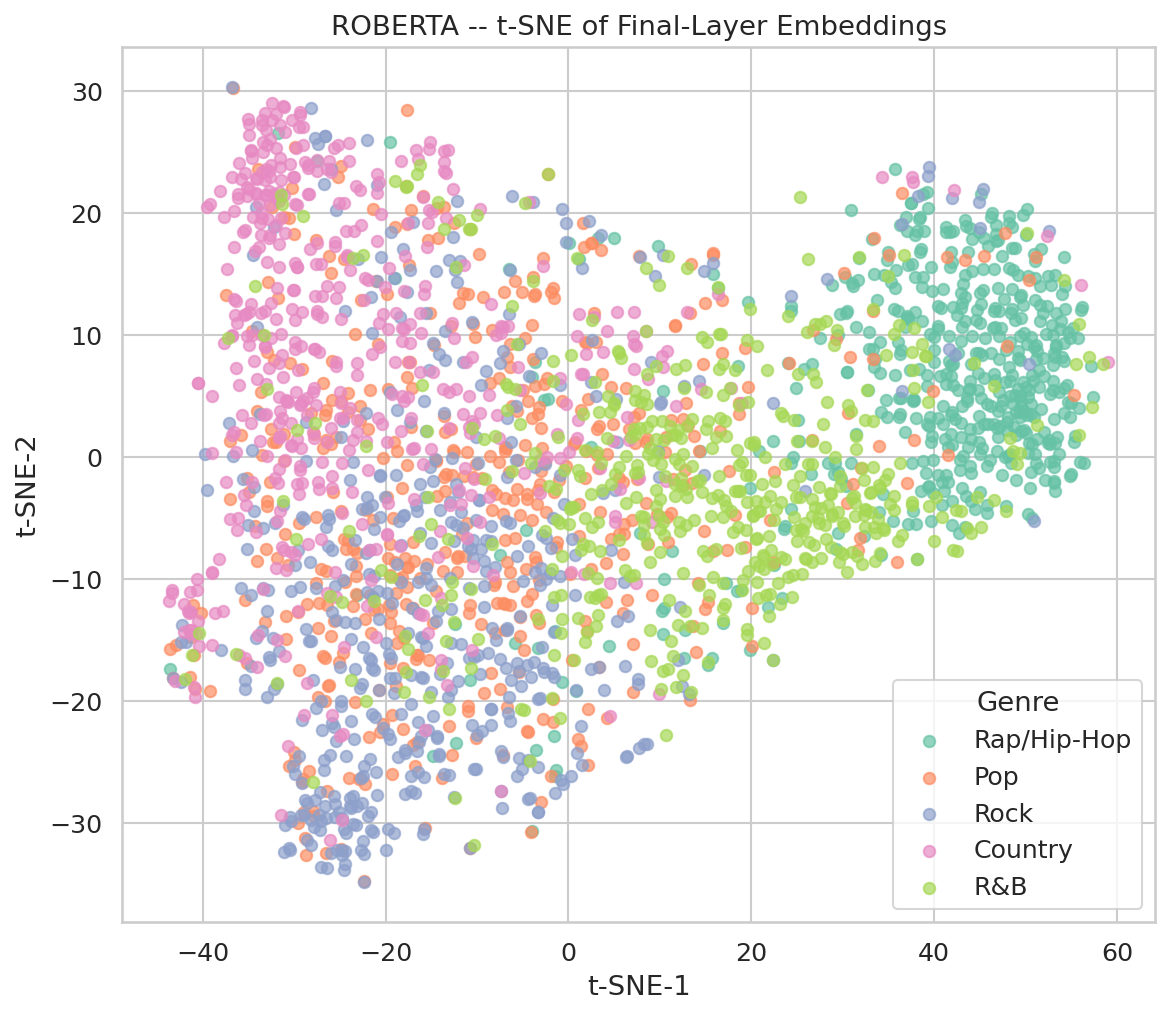
\includegraphics[width=\textwidth]{t-sne_roberta.png}
    \caption{t-SNE projection.}
  \end{subfigure}
  \caption{2D projections of RoBERTa final-layer \texttt{[CLS]}
  embeddings. Rap and Country form relatively tight clusters; Pop,
  Rock, and R\&B are heavily interleaved.}
  \label{fig:embeddings}
\end{figure}

Both UMAP and t-SNE projections (Figure~\ref{fig:embeddings}) of the
learned \texttt{[CLS]} representations visually confirm the
quantitative findings.
Rap forms the most distinct cluster, consistent with its unique
vocabulary.
Country clusters reasonably well.
However, Pop, Rock, and R\&B are heavily interleaved, visualizing the
genre boundary ambiguity that limits performance.

\subsection{Layer Probing: Genre Is a Mid-Level Property}

\begin{figure}[t]
  \centering
  \begin{subfigure}[b]{0.48\textwidth}
    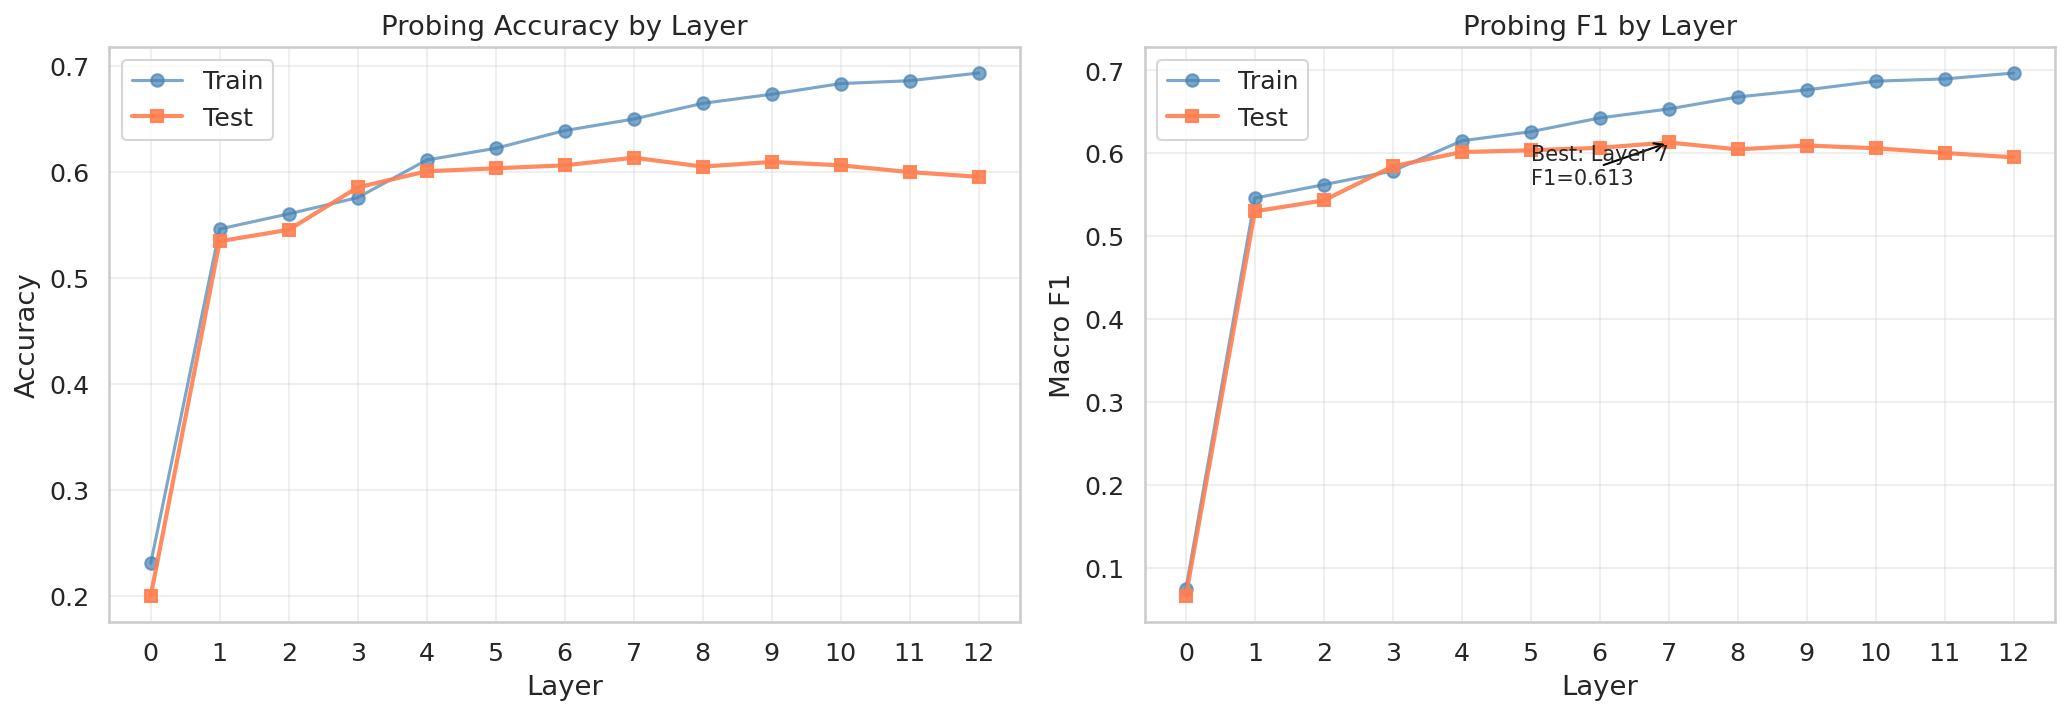
\includegraphics[width=\textwidth]{layer_probing.png}
    \caption{Overall accuracy and F1 by layer.}
    \label{fig:lp_overall}
  \end{subfigure}
  \hfill
  \begin{subfigure}[b]{0.48\textwidth}
    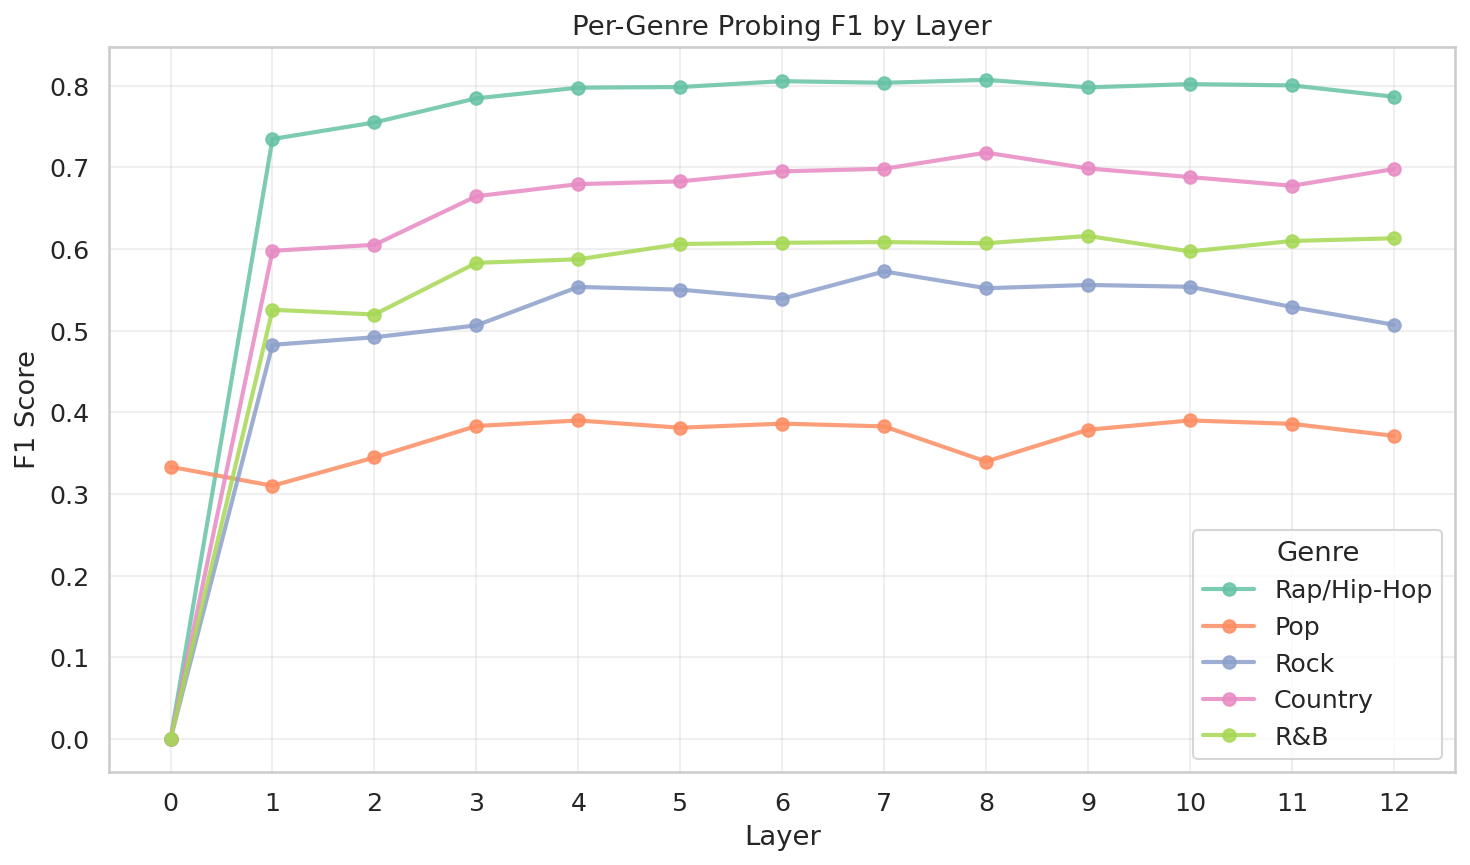
\includegraphics[width=\textwidth]{layer_probing_per_genre.png}
    \caption{Per-genre F1 by layer.}
    \label{fig:lp_genre}
  \end{subfigure}
  \caption{Layer probing results. Genre information is absent at
  layer~0 (F1\,=\,0.067), jumps dramatically at layer~1 (0.530),
  improves through layer~7 (0.613), then plateaus.}
  \label{fig:layer_probing}
\end{figure}

Layer probing (Figure~\ref{fig:layer_probing}) reveals the trajectory of
genre information through the network:

\begin{itemize}[leftmargin=*,itemsep=1pt]
\item \textbf{Layer~0} (static embeddings): F1\,=\,0.067---barely
  above random.
  Word embeddings alone carry negligible genre signal.
\item \textbf{Layer~1}: F1 jumps to 0.530.
  A single transformer block integrates enough contextual information
  for basic genre discrimination.
\item \textbf{Layers~2--7}: Steady improvement to F1\,=\,0.613
  at layer~7 (the peak).
\item \textbf{Layers~8--12}: Plateau, with the final layer at
  F1\,=\,0.595---slightly \emph{below} the peak.
\end{itemize}

\noindent
This trajectory suggests that genre is a \emph{mid-level linguistic
property}: deeper than bag-of-words (layer~0 fails) but shallower than
the abstract semantic reasoning built in deeper layers.
The plateau after layer~7 is a \textbf{representational ceiling}:
additional depth does not improve genre discrimination because the
model has already extracted all linearly accessible signal from the
input.
This is an \emph{information} ceiling, not a model capacity ceiling.

The per-genre breakdown (Figure~\ref{fig:lp_genre}) shows that Rap is
classifiable from the earliest layers (its vocabulary is highly
distinctive), while Pop remains the hardest genre throughout all layers
(per-class F1~$\approx$~0.38), consistent with its weak TF-IDF
signature and high overlap with other genres.

\subsection{Contrastive Integrated Gradients: What Little Signal Exists}

\begin{figure}[t]
  \centering
  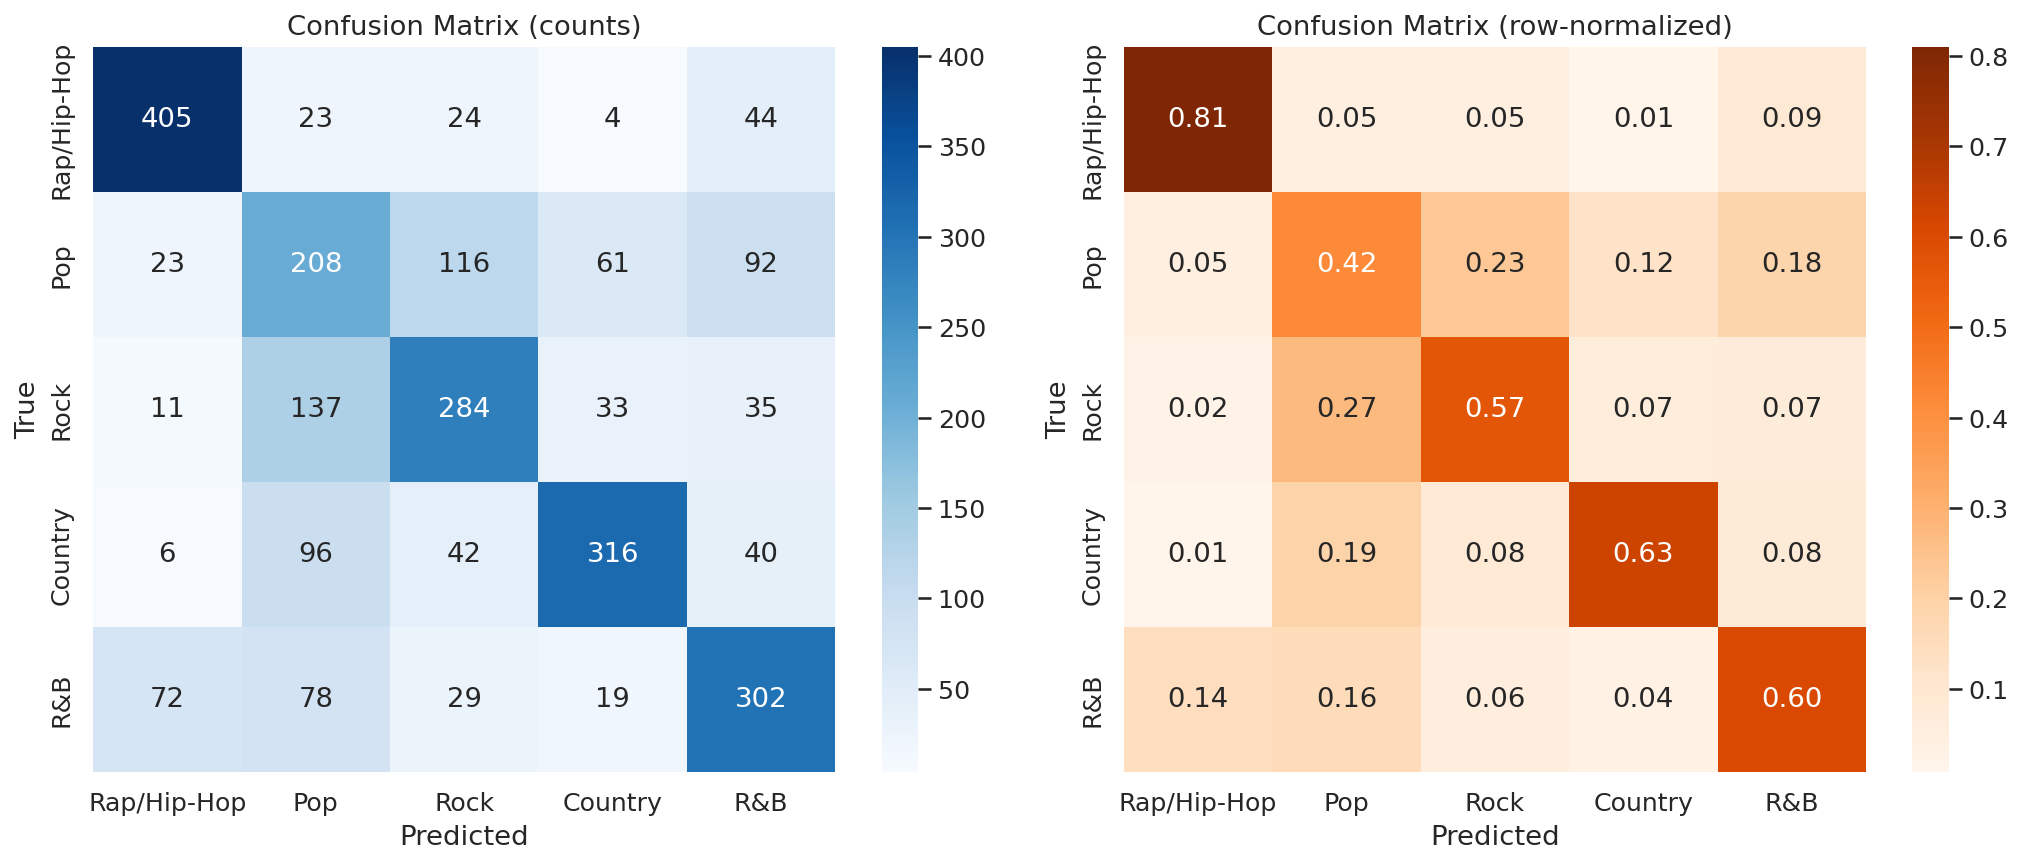
\includegraphics[width=0.65\textwidth]{contrastive/confusion_analysis.png}
  \caption{Confusion counts and per-class accuracy for the
  RoBERTa interpretability model, identifying the top confused pairs.}
  \label{fig:contrastive_cm}
\end{figure}

The top confused pairs are identified from the confusion matrix
(Figure~\ref{fig:contrastive_cm}).
Standard Integrated Gradients answer \emph{which tokens matter for
predicting genre~A}; contrastive IG answers \emph{which tokens push
the model toward A rather than B}.
This distinction is critical when genres overlap: a token like
``love'' has high standard IG for both Pop and Country, but near-zero
\emph{contrastive} attribution for the Pop-vs.-Country pair.

For Rock~vs.~Pop, tokens associated with intense themes
(\emph{death}, \emph{blood}, \emph{pain}) push toward Rock, while
lighter emotional vocabulary (\emph{love}, \emph{night}, \emph{feel})
pushes toward Pop.
Misclassifications occur when a Rock song uses softer language or a
Pop song employs darker imagery---genuine lyrical ambiguity.

For Country~vs.~Pop, the model relies on rural/domestic terms
(\emph{truck}, \emph{town}, \emph{mama}) to identify Country, but
Country-Pop crossover songs often lack these markers.
These findings confirm that the model has learned reasonable
genre-discriminating features and that errors arise from genuine
ambiguity rather than model failure.


% ══════════════════════════════════════════════════════════════════════════════
\section{Discussion}
\label{sec:discussion}

\subsection{The Performance Ceiling}
\label{sec:ceiling}

The central finding of this work is that lyrics-only genre
classification is bounded at approximately F1\,$\approx$\,0.65.
Four converging lines of evidence support this conclusion:

\begin{enumerate}[leftmargin=*,itemsep=2pt]
\item \textbf{Genre similarity:} Pop--Rock centroid cosine similarity
  is 0.979 (Sentence-BERT), and within/between-genre distributions
  overlap almost entirely.
  These genres are distinguished primarily by musical properties
  (instrumentation, tempo, production) that lyrics do not capture.
\item \textbf{Layer probing plateau:} Genre information saturates by
  layer~7, meaning the model has extracted all linearly accessible
  signal by mid-depth.
  This is an information ceiling, not a model capacity ceiling.
\item \textbf{Error--similarity correlation:} Model confusion mirrors
  genre proximity ($r = 0.630$), confirming errors arise from data
  structure, not model failure.
\item \textbf{LLM upper bound:} Claude~Opus---a frontier LLM with
  world knowledge of artists and musical context---achieves only
  F1\,=\,0.636 in zero-shot mode, only 2.5~points above our
  fine-tuned RoBERTa.
\end{enumerate}

\noindent
The marginal gain from world knowledge (0.636 vs.\ 0.611) suggests
that the classification task is fundamentally constrained by the
lyrics modality, not by the model's knowledge or capacity.

\subsection{Scaling Does Not Help}

The interpretability RoBERTa, trained on 2.5$\times$ more data per genre
with augmentation, achieves F1\,=\,0.608---essentially identical to the
comparison RoBERTa (0.611).
This is consistent with the ceiling hypothesis: if the input lacks
discriminative content, neither more data nor more capacity will help.
We note, however, that this Phase~2 experiment changed multiple
variables simultaneously (data size, learning rate, augmentation, LoRA
targets), so the null improvement cannot be attributed to any single
factor.

\subsection{Architectural Differences vs.\ Confounds}

RoBERTa's advantage over GPT-2 (2~points~F1) is consistent with
bidirectional attention benefiting document-level classification: the
\texttt{[CLS]} token can attend to genre cues at arbitrary positions,
whereas GPT-2's causal mask forces incremental left-to-right
accumulation.
However, this comparison is confounded by the $150\times$ larger
trainable classification head (594K vs.\ 3.8K).

T5's larger gap ($-$15~points) is likely multi-causal:
(1)~the smaller base model (\texttt{t5-small} at 60M vs.\ 125M) starts
with weaker representations;
(2)~the text-to-text formulation adds unnecessary decoding overhead for
a classification task;
and (3)~T5's language model head is frozen, so all adaptation occurs
through LoRA alone.
A fairer comparison would use \texttt{t5-base} (220M) and equalize
head sizes.

\subsection{Limitations}
\label{sec:limitations}

\begin{itemize}[leftmargin=*,itemsep=2pt]
\item \textbf{No multi-seed variance reporting.}
  All results are single-run point estimates.
  The 2-point F1 gap between RoBERTa and GPT-2 could be within noise.
  Confidence intervals from multiple random seeds would strengthen or
  qualify the architectural comparison.

\item \textbf{Unequal comparison conditions.}
  The three models differ in base size (60M vs.\ 125M), total trainable
  parameters (0.59M vs.\ 1.18M), and head design.
  While LoRA adapters are matched (590K), the overall trainable budget
  is not.

\item \textbf{No human performance baseline.}
  Without measuring inter-annotator agreement on lyrics-only genre
  labeling, we cannot distinguish ``the task is inherently hard'' from
  ``the genre labels are noisy.''

\item \textbf{Dataset quality.}
  The Genius dataset contains noise: spam entries, non-lyrical content,
  and metadata artifacts (see the EDA sample revealing a product
  description labeled as ``Rock'').

\item \textbf{Character truncation.}
  The 2{,}000-character limit disproportionately truncates Rap lyrics
  (median at the cap), potentially removing genre-distinctive content.

\item \textbf{Genre taxonomy.}
  Five broad genres is a coarse taxonomy.
  Finer-grained labels or hierarchical classification could yield
  different conclusions.

\item \textbf{LLM sample size.}
  The Claude evaluation uses 250 samples, introducing higher variance
  ($\pm$6\% per-class F1 at 95\% confidence) than the full test set.
\end{itemize}


% ══════════════════════════════════════════════════════════════════════════════
\section{Conclusion}
\label{sec:conclusion}

We compared three transformer architectures for lyrics-based music
genre classification under LoRA fine-tuning.
RoBERTa achieved the highest macro~F1 (0.611), though confounded
by a larger classification head; GPT-2 followed closely (0.591);
and T5 underperformed (0.463), partly due to its smaller base model.
These rankings reflect the full experimental setup rather than purely
architectural differences.

More importantly, we established through four converging
analyses---genre similarity, layer probing, error--similarity
correlation, and embedding visualization---that lyrics-only
classification has an inherent performance ceiling of approximately
F1\,$\approx$\,0.65.
This ceiling is data-driven: genres like Pop and Rock are linguistically
near-identical (centroid cosine similarity 0.979) and are distinguished
primarily by musical properties that lyrics cannot capture.
Even Claude~Opus, a frontier LLM with world knowledge, achieves only
0.636.

The contrastive Integrated Gradients analysis reveals that when the
model does fail, it fails \emph{rationally}: errors occur precisely
where lyrics are genuinely ambiguous between genres.
This is the core insight: when an information ceiling has been reached,
the path forward is not more data or model capacity but richer input
modalities.
Future work should explore multimodal approaches combining lyrics
with audio features to break through this text-only ceiling.


% ══════════════════════════════════════════════════════════════════════════════
\bibliographystyle{plainnat}
\bibliography{references}

\end{document}
